%%%%% DO IN R INSTEAD!!!!!!

\documentclass[class=minimal, border = 0pt, crop]{standalone}
\usepackage{pgf}
\usepackage{tikz}
\usepackage[utf8]{inputenc}
\usepackage{amsmath}
\usepackage{amsthm}
\DeclareMathAlphabet\mathbb{U}{msb}{m}{n}
\usetikzlibrary{arrows,automata,shapes,calc,backgrounds,decorations.pathreplacing,snakes}
\usetikzlibrary{positioning}
\pagestyle{empty}
\tikzset{
    state/.style={
           rectangle,
           rounded corners,
           draw=blue!50, very thick,
           minimum height=2em,
           inner sep=5pt,
           text centered,
           },
    pil/.style={
           ->,
           thick,
           shorten <=4pt,
           shorten >=4pt,
           },
    ball/.style={
           circle,
           draw,
           align=center,
           anchor=north,
           inner sep=0,
           fill=blue!50,
           }
}

\begin{document}
\centering
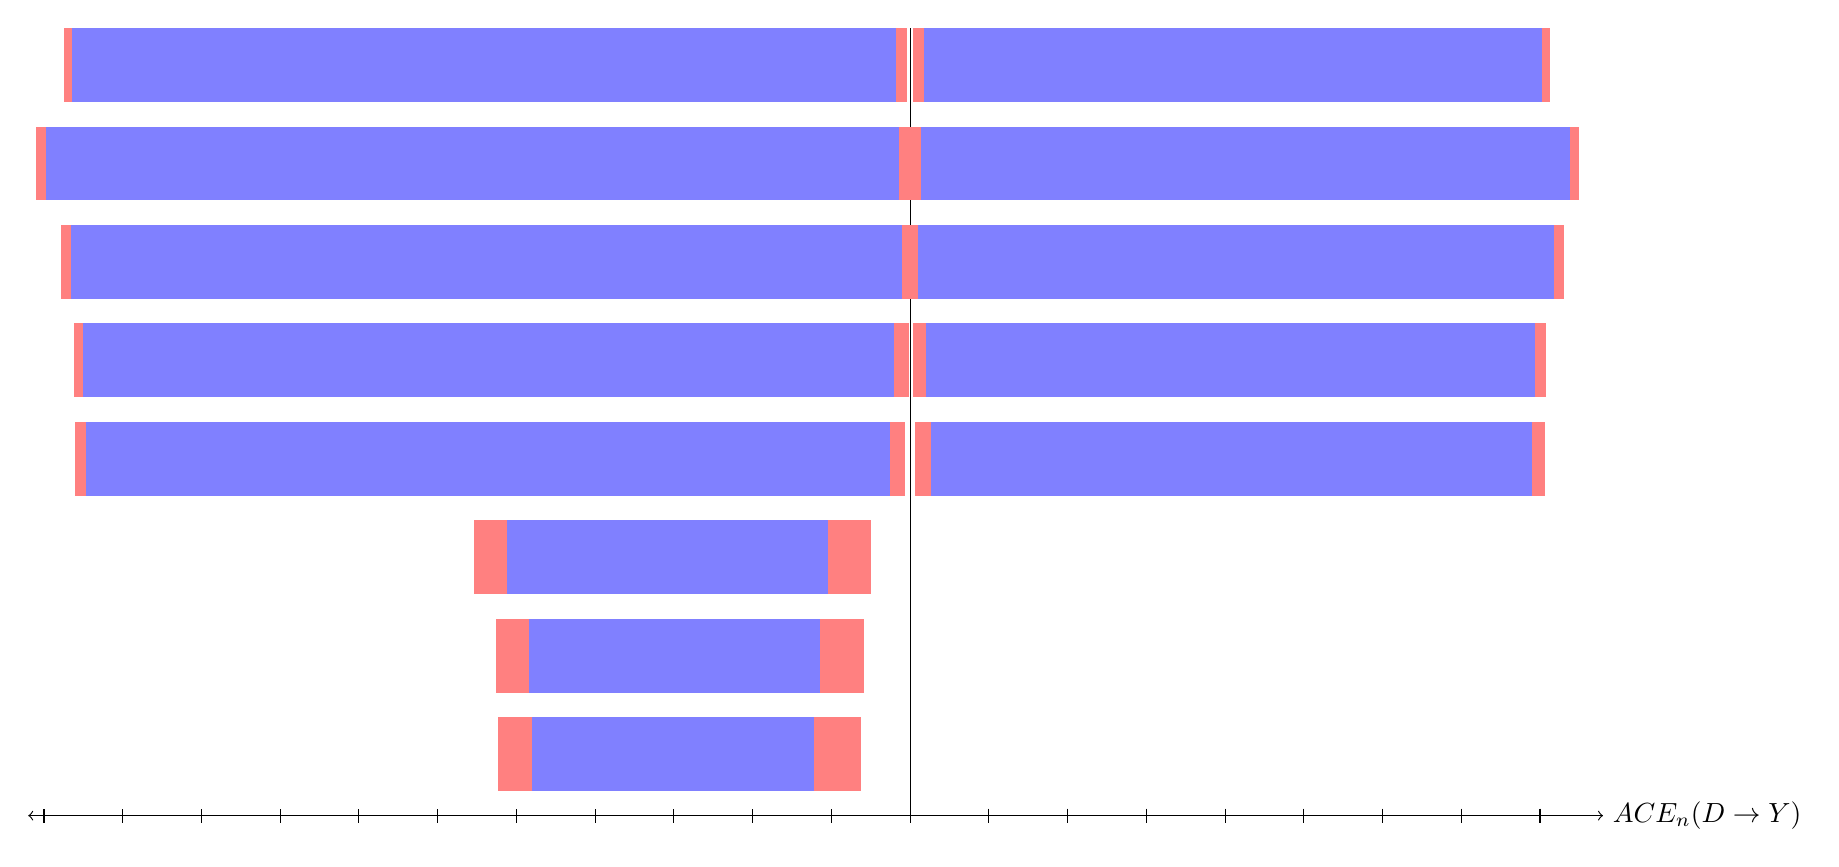
\begin{tikzpicture}
 \coordinate (O) at (0,0);
  \draw[<->] (-11.2,0) -- (8.8,0) coordinate[label = {right:$ACE_n(D\rightarrow Y)$}] (xmax);
  \draw[] (0,0) -- (0,10) coordinate[] (ymax);
%8
  \draw[fill=red!50,draw=none] (-0.262*20,0.1*10/3.2) rectangle (-0.031*20,0.4*10/3.2);
  \draw[fill=blue!50,draw=none] (-0.240*20,0.1*10/3.2) rectangle (-0.061*20,0.4*10/3.2);
%7  
 \draw[fill=red!50,draw=none] (-0.263*20,0.5*10/3.2) rectangle (-0.029*20,0.8*10/3.2);
  \draw[fill=blue!50,draw=none] (-0.242*20,0.5*10/3.2) rectangle (-0.057*20,0.8*10/3.2);
  %6
 \draw[fill=red!50,draw=none] (-0.277*20,0.9*10/3.2) rectangle (-0.025*20,1.2*10/3.2);
  \draw[fill=blue!50,draw=none] (-0.256*20,0.9*10/3.2) rectangle (-0.052*20,1.2*10/3.2);
  %5a
 \draw[fill=red!50,draw=none] (-0.530*20,1.3*10/3.2) rectangle (-0.003*20,1.6*10/3.2);
  \draw[fill=blue!50,draw=none] (-0.523*20,1.3*10/3.2) rectangle (-0.013*20,1.6*10/3.2);
  %4a
 \draw[fill=red!50,draw=none] (-0.531*20,1.7*10/3.2) rectangle (-0.001*20,2*10/3.2);
  \draw[fill=blue!50,draw=none] (-0.525*20,1.7*10/3.2) rectangle (-0.010*20,2*10/3.2);
  %3a
 \draw[fill=red!50,draw=none] (-0.539*20,2.1*10/3.2) rectangle (0.003*20,2.4*10/3.2);
  \draw[fill=blue!50,draw=none] (-0.533*20,2.1*10/3.2) rectangle (-0.005*20,2.4*10/3.2);
  %2a
 \draw[fill=red!50,draw=none] (-0.555*20,2.5*10/3.2) rectangle (0.001*20,2.8*10/3.2);
  \draw[fill=blue!50,draw=none] (-0.549*20,2.5*10/3.2) rectangle (-0.007*20,2.8*10/3.2);
  %1a
 \draw[fill=red!50,draw=none] (-0.537*20,2.9*10/3.2) rectangle (-0.002*20,3.2*10/3.2);
  \draw[fill=blue!50,draw=none] (-0.532*20,2.9*10/3.2) rectangle (-0.009*20,3.2*10/3.2);
  %5b
 \draw[fill=red!50,draw=none] (0.003*20,1.3*10/3.2) rectangle (0.403*20,1.6*10/3.2);
  \draw[fill=blue!50,draw=none] (0.013*20,1.3*10/3.2) rectangle (0.395*20,1.6*10/3.2);
  %4b
 \draw[fill=red!50,draw=none] (0.002*20,1.7*10/3.2) rectangle (0.404*20,2*10/3.2);
  \draw[fill=blue!50,draw=none] (0.010*20,1.7*10/3.2) rectangle (0.397*20,2*10/3.2);
  %3b
 \draw[fill=red!50,draw=none] (-0.003*20,2.1*10/3.2) rectangle (0.415*20,2.4*10/3.2);
  \draw[fill=blue!50,draw=none] (0.005*20,2.1*10/3.2) rectangle (0.409*20,2.4*10/3.2);
  %2b
 \draw[fill=red!50,draw=none] (-0.001*20,2.5*10/3.2) rectangle (0.425*20,2.8*10/3.2);
  \draw[fill=blue!50,draw=none] (0.007*20,2.5*10/3.2) rectangle (0.419*20,2.8*10/3.2);
  %1b
\draw[fill=red!50,draw=none] (0.002*20,2.9*10/3.2) rectangle (0.406*20,3.2*10/3.2);
  \draw[fill=blue!50,draw=none] (0.009*20,2.9*10/3.2) rectangle (0.401*20,3.2*10/3.2);
   \draw[snake=ticks,segment length=1cm] (0,0) -- (8.8,0);
      \draw[snake=ticks,segment length=1cm] (0,0) -- (-11.2,0);
\end{tikzpicture}
\end{document}